%%----------------------------------------------------------------------------------------
\clearpage
\pagestyle{fancy}
%%----------------------------------------------------------------------------------------
%%       PREFAZIONE
%%----------------------------------------------------------------------------------------
\part{Carichi ripartiti su una trave}
\setcounter{section}{0}
\section{Carico trasversale e carico assiale per unità di lunghezza}
%----------------------------------------------------------------------------------------
%--------------------------------------------------------------------------------------------------------------------------------------------------------------
\renewcommand{\thefigure}{10~-~1}
\begin{figure}[ht]
\centering
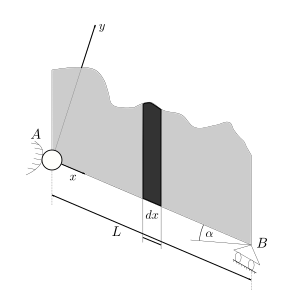
\includegraphics[width=0.65\textwidth]{Immagini/Parte_10/Figura10_1/figura10_1.pdf}
\caption{}
\label{figura10-1}
\end{figure}
%--------------------------------------------------------------------------------------------------------------------------------------------------------------
In figura~\ref{figura10-1} è rappresentata una trave rettilinea il cui asse forma un angolo $\alpha$ con l'orizzontale. In questo capitolo e nei successivi assumeremo la seguente terna di riferimento levogira: $x$ asse coincidente con l'asse della trave, $y$ ortogonale ad $x$ giacente nel piano in cui agiscono le forze (ed è orientato in modo tale che $x$ debba ruotare di $90^{\circ}$ in senso antiorario per sovrapporsi ad esso) e $z$ completa la terna levogira (in figura esso è uscente). Immaginiamo che sulla trave vi sia un \emph{muro rotto} di spessore costante. Esso, ovviamente, grava sulla trave esercitando su di essa un carico verticale; il suddetto carico, evidentemente, non è assimilabile ad una forza concentrata: si può dire che il peso del muro è \textbf{distribuito} lungo l'asse della trave. Più in dettaglio: su ogni tratto infinitesimo $dx$ di trave agisce una forza infinitesima $dF$ pari al peso della striscetta di muro (ombreggiata in figura) che sovrasta il tratto $dx$ in questione. Detta $h$ l'altezza della striscetta suddetta, $b$ lo spessore del muro (non visibile in figura) e $\gamma$ il peso specifico del materiale di cui il muro è fatto, risulta ovviamente:
%----------------------------------------------------------------------------------------
\begin{equation} \label{equazione10-1}
dF = \text{Peso specifico} \times \text{Volume} = \gamma\cdot b\cdot h\cdot \cos{\alpha}\cdot dx \tag{10.1}
\end{equation}
%----------------------------------------------------------------------------------------
Poniamo 
%----------------------------------------------------------------------------------------
\begin{equation*}
\boxed{\gamma \cdot b \cdot h \cos{\alpha} = q}
\end{equation*}
%----------------------------------------------------------------------------------------
ed osserviamo che, essendo $\gamma$, $b$ e $\cos{\alpha}$ costanti con $x$, la funzione $q = q(x)$ è proporzionale alla funzione $h = h(x)$ ed il suo grafico è praticamente simile alla \emph{sagoma del muro}. Poiché risulta ovviamente 
%----------------------------------------------------------------------------------------
\begin{equation*}
\boxed{dF = q \cdot dx}
\end{equation*}
%----------------------------------------------------------------------------------------
e quindi
%----------------------------------------------------------------------------------------
\begin{equation*}
\boxed{q = \frac{dF}{dx}}
\end{equation*}
%----------------------------------------------------------------------------------------
$q$ prende il nome di \textsc{carico per unità di lunghezza} ed il suo grafico viene detto \textsc{diagramma di carico}; le dimensioni fisiche di $q$ sono ovviamente quelle di una forza per unità di lunghezza ($[F \cdot L^{-1}]$). Le componenti del vettore $\underline{q}$ nelle direzioni $x$ ed $y$ prendono rispettivamente il nome di \textbf{carico assiale} e \textbf{carico trasversale}; essi si assumono positive se concordi con i corrispondenti assi. 
%--------------------------------------------------------------------------------------------------------------------------------------------------------------
\renewcommand{\thefigure}{10~-~2}
\begin{figure}[ht]
\centering
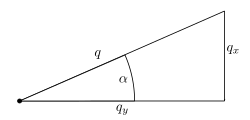
\includegraphics[width=0.55\textwidth]{Immagini/Parte_10/Figura10_2/figura10_2.pdf}
\caption{}
\label{figura10-2}
\end{figure}
%--------------------------------------------------------------------------------------------------------------------------------------------------------------
Con riferimento alla figura~\ref{figura10-2}:
%----------------------------------------------------------------------------------------
\begin{align}
q_x &= q\cdot \sin{\alpha} = q_a \label{equazione10.2a} \tag{10.2a}\\ 
q_y &= q\cdot \cos{\alpha} = q_t \label{equazione10.2b} \tag{10.2b}
\end{align}
%----------------------------------------------------------------------------------------
Essendo $\alpha$ costante, $q_x$ e $q_y$ hanno la legge di variazione proporzionale a quella di $q$ e, di conseguenza, diagrammi simili.
%----------------------------------------------------------------------------------------
\section{La risultante del carico ripartito}
%----------------------------------------------------------------------------------------
%--------------------------------------------------------------------------------------------------------------------------------------------------------------
\renewcommand{\thefigure}{10~-~3}
\begin{figure}[ht]
\centering
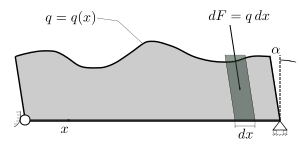
\includegraphics[width=0.65\textwidth]{Immagini/Parte_10/Figura10_3/figura10_3.pdf}
\caption{}
\label{figura10-3}
\end{figure}
%--------------------------------------------------------------------------------------------------------------------------------------------------------------
In figura~\ref{figura10-3} è rappresentata una trave rettilinea soggetta ad un carico ripartito $q$ che forma l'angolo $\alpha$ con l'asse $y$. Non è necessario specificare la natura del carico, che potrebbe essere gravitazionale, inerziale, aerodinamico e così via. Il messaggio che deve essere recepito dalle figure e è il seguente: \textbf{su ogni segmento} $dx$ \textbf{della trave agisce una forza infinitesima} $dF = q\cdot dx$ \textbf{avente direzione e verso di} $q$. È preferibile considerare separatamente le componenti assale e trasversale di $q$.
%--------------------------------------------------------------------------------------------------------------------------------------------------------------
\renewcommand{\thefigure}{10~-~4}
\begin{figure}[ht]
\centering
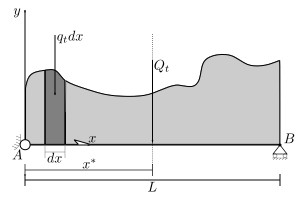
\includegraphics[width=0.65\textwidth]{Immagini/Parte_10/Figura10_4/figura10_4.pdf}
\caption{}
\label{figura10-4}
\end{figure}
%--------------------------------------------------------------------------------------------------------------------------------------------------------------
Cominciamo dal carico trasversale; osservando la figura~\ref{figura10-4}, la risultante di tutte le forze elementari $q_{t}\cdot dx$ è detta \textsc{risultante del carico trasversale} e viene indicata con $Q_{t}$. Essa ha ovviamente direzione e verso di $q_{t}$ ed il suo modulo vale
%----------------------------------------------------------------------------------------
\begin{equation} \label{equazione10-3}
\boxed{ Q_{t} = \int_{0}^{L} q_{t}\,dx = \text{Area del diagramma di carico}} \tag{10.3}
\end{equation}
%----------------------------------------------------------------------------------------
Per determinare la retta di azione di $Q_{t}$ facciamo uso del \textsc{teorema di Varignon}; scelto $A$ come polo, abbiamo
%----------------------------------------------------------------------------------------
\begin{equation*}
Q_{t} \cdot x^{*} = \int_{0}^{L} q_{t}\cdot x\,dx
\end{equation*}
%----------------------------------------------------------------------------------------
da cui si ricava immediatamente
%----------------------------------------------------------------------------------------
\begin{equation} \label{10-4}
\boxed{ x^{*} = \frac{ \int_{0}^{L} q_{t}\cdot x\,dx }{Q_{t}} } \tag{10.4}
\end{equation}
%----------------------------------------------------------------------------------------
Si osservi che il termine $\int_{0}^{L} q_{t}\cdot x\,dx$ rappresenta il \textsc{momento statico}, calcolato rispetto ad $y$, del diagramma di carico; $Q_{t}$, come è noto, rappresenta l'area del diagramma di carico e, pertanto, $x^{*}$ altro non è che l'\textsc{ascissa del baricentro del diagramma di carico}. Possiamo dunque ritenere dimostrata la seguente proposizione:
%--------------------------------------------------------------------------------------------------------------------------------------------------------------
\\

\fbox{\begin{minipage}{38em}
\centering
\textsc{La risultante di un carico trasversale ha modulo uguale all'area del diagramma di carico e passa per il suo baricentro.}
\end{minipage}}\\
%--------------------------------------------------------------------------------------------------------------------------------------------------------------

\noindent Per quanto riguarda il carico assiale, dovrebbe essere ovvia a questo punto la seguente proposizione:
%--------------------------------------------------------------------------------------------------------------------------------------------------------------
\\

\fbox{\begin{minipage}{38em}
\centering
\textsc{La risultante di un carico assiale ha modulo uguale all'area del diagramma di carico; la sua retta d'azione coincide con l'asse $x$ poiché tutte le forze elementari $q_{a}\cdot dx$ agiscono lungo l'asse $x$.}
\end{minipage}}
%--------------------------------------------------------------------------------------------------------------------------------------------------------------
%--------------------------------------------------------------------------------------------------------------------------------------------------------------
\clearpage
\section{Esercizi}
\paragraph{Esercizio 10.1}
%--------------------------------------------------------------------------------------------------------------------------------------------------------------
\renewcommand{\thefigure}{10.1~-~1}
\begin{figure}[ht]
\centering
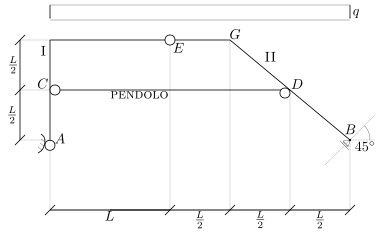
\includegraphics[width=0.75\textwidth]{Immagini/Parte_10/Esercizio10_1_1/Esercizio10_1_1.pdf}
\caption{}
\label{Esercizio10-1-1}
\end{figure}
%--------------------------------------------------------------------------------------------------------------------------------------------------------------
%----------------------------------------------------------------------------------------
Si chiede di
%----------------------------------------------------------------------------------------
\begin{enumerate}
\item classificare la struttura assegnata; 
\item calcolare le reazioni vincolari, a patto che essa sia in equilibrio e sia staticamente determinata; 
\item di valutare $q_{t}$ e $q_{a}$ sul tratto $GB$.
\end{enumerate}
%----------------------------------------------------------------------------------------
\subparagraph{Quesito 1}
%----------------------------------------------------------------------------------------
La struttura è costituita da due tronchi, poiché $CD$ lo consideriamo pendolo. Dunque:
%----------------------------------------------------------------------------------------
\begin{align*}
m &= 2\times 3 = 6 \\ 
n &= 2A + 1B + 1p + 2E = 6
\end{align*}
%----------------------------------------------------------------------------------------
per cui si ricava 
%----------------------------------------------------------------------------------------
\begin{equation*}
m - n = l - i = 0
\end{equation*}
%----------------------------------------------------------------------------------------
Risulta evidente che $(1, 2)$ non esiste; ciò vuol dire che i due tronchi sono solidali. D'altra parte, il blocco rigido formato dai due tronchi non può muoversi e per comprenderlo basta guardare la cerniera in $A$ ed il carrello in $B$. Dunque, in definitiva $l=0$, $i=0$ e la struttura è \textsc{isostatica}. 
%----------------------------------------------------------------------------------------
\subparagraph{Quesito 2}
%----------------------------------------------------------------------------------------
%--------------------------------------------------------------------------------------------------------------------------------------------------------------
\renewcommand{\thefigure}{10.1~-~2}
\begin{figure}[ht]
\centering
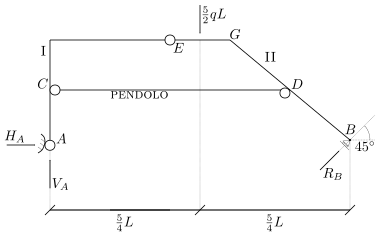
\includegraphics[width=0.75\textwidth]{Immagini/Parte_10/Esercizio10_1_1/Esercizio10_1_2.pdf}
\caption{}
\label{Esercizio10-1-2}
\end{figure}
%--------------------------------------------------------------------------------------------------------------------------------------------------------------
Essendo la struttura isostatica per vincoli esterni, cominciamo ad imporre l'equilibrio esterno; in questa fase è lecito ed opportuno sostituire al carico distribuito la sua risultante:
%----------------------------------------------------------------------------------------
\begin{subequations}
\begin{align}
H_{A} + \frac{\sqrt{2}}{2}R_{B} &= 0 \quad [\rightarrow] \label{equazione10-1-1a} \tag{10.1.1a} \\
V_{A} + \frac{\sqrt{2}}{2}R_{B} - \frac{5}{2} qL &= 0 \quad [\uparrow] \label{equazione10-1-1b} \tag{10.1.1b} \\ 
-V_{A}\frac{5}{2}L + \frac{5}{2}qL \cdot \frac{5}{4}L &= 0 \quad [B\, \circlearrowleft] \label{equazione10-1-1c} \tag{10.1.1c}
\end{align}
\end{subequations}
%----------------------------------------------------------------------------------------
Quindi, si ricava quanto segue:
%----------------------------------------------------------------------------------------
\begin{subequations}
\begin{align}
V_{A} &= \frac{5}{4}qL  \quad [\uparrow] \label{equazione10-1-2a} \tag{10.1.2a} \\
R_{B} &= \frac{5\sqrt{2}}{2}qL - \sqrt{2}V_{A} = \frac{5\sqrt{2}}{2}qL - \frac{5\sqrt{2}}{4}qL = \frac{5\sqrt{2}}{4}qL \quad [\nearrow] \label{equazione10-1-2b} \tag{10.1.2b} \\ 
H_{A} &= -\frac{\sqrt{2}}{2}R_{B} = \frac{5\sqrt{2}}{8}\cdot \sqrt{2} qL = - \frac{5}{4}qL \quad [\leftarrow] \label{equazione10-1-2c} \tag{10.1.2c}
\end{align}
\end{subequations}
%----------------------------------------------------------------------------------------
%--------------------------------------------------------------------------------------------------------------------------------------------------------------
\renewcommand{\thefigure}{10.1~-~3}
\begin{figure}[ht]
\centering
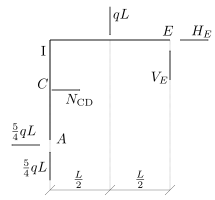
\includegraphics[width=0.75\textwidth]{Immagini/Parte_10/Esercizio10_1_1/Esercizio10_1_3.pdf}
\caption{}
\label{Esercizio10-1-3}
\end{figure}
%--------------------------------------------------------------------------------------------------------------------------------------------------------------
A questo punto, note $H_{A}$, $V_{A}$ ed $R_{B}$, entrambi i tronchi risultano statisticamente determinati. Andiamo ad imporre l'equilibrio del primo tronco. Ora che disegneremo il primo tronco isolato, considereremo, ovviamente, la risultante della sola parte di carico che gli compete; il primo tronco è rappresentato in figura~\ref{Esercizio10-1-3}: 
%----------------------------------------------------------------------------------------
\begin{subequations}
\begin{align}
-\frac{5}{4}qL + N_{\textup{CD}} + H_{E} &= 0 \quad [\rightarrow] \label{equazione10-1-3a} \tag{10.1.3a} \\
\frac{5}{4}qL - qL + V_{E} &= 0 \quad [\uparrow] \label{equazione10-1-3b} \tag{10.1.3b} \\ 
-\frac{5}{4}qL\cdot L - -\frac{5}{4}qL \cdot L + N_{\textup{CD}}\cdot \frac{L}{2} + qL \cdot \frac{L}{2} &= 0 \quad [E\, \circlearrowleft] \label{equazione10-1-3c} \tag{10.1.3c}
\end{align}
\end{subequations}
%----------------------------------------------------------------------------------------
e, dunque, risolvendo il sistema
%----------------------------------------------------------------------------------------
\begin{subequations}
\begin{align}
N_{\textup{CD}} &= 4qL \quad [\text{Tirante}] \label{equazione10-1-4a} \tag{10.1.4a} \\
V_{E} &= -\frac{qL}{4} \quad [\downarrow] \label{equazione10-1-4b} \tag{10.1.4b} \\ 
H_{E} &= -\frac{11}{4}qL \quad [\leftarrow] \label{equazione10-1-4c} \tag{10.1.4c}
\end{align}
\end{subequations}
%----------------------------------------------------------------------------------------
%--------------------------------------------------------------------------------------------------------------------------------------------------------------
\renewcommand{\thefigure}{10.1~-~4}
\begin{figure}[ht]
\centering
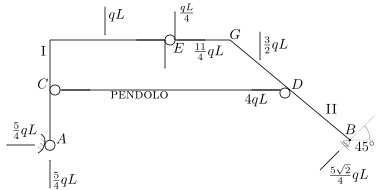
\includegraphics[width=0.75\textwidth]{Immagini/Parte_10/Esercizio10_1_1/Esercizio10_1_4.pdf}
\caption{}
\label{Esercizio10-1-4}
\end{figure}
%--------------------------------------------------------------------------------------------------------------------------------------------------------------
In figura~\ref{Esercizio10-1-4} è rappresentato il quadro completo delle reazioni. Possiamo legittimare i risultati controllando che il secondo tronco sia in equilibrio:
%----------------------------------------------------------------------------------------
\begin{subequations}
\begin{align}
\frac{5}{4}qL - 4qL + \frac{11}{4}qL &= 0 \quad [\text{Ok}] \label{equazione10-1-5a} \tag{10.1.5a} \\
\frac{qL}{4} - \frac{3}{2}qL + \frac{5}{4} qL &= 0 \quad [\text{Ok}] \label{equazione10-1-5b} \tag{10.1.5b} \\ 
\frac{5}{4}qL \cdot L + \frac{5}{4} qL \cdot \frac{3}{4} L - 4qL\cdot \frac{L}{2} - \frac{3}{2}qL \cdot \frac{3}{4} L &= 0 \quad [\text{Ok}] \label{equazione10-1-5c} \tag{10.1.5c}
\end{align}
\end{subequations}
%----------------------------------------------------------------------------------------
\subparagraph{Quesito 3}
%--------------------------------------------------------------------------------------------------------------------------------------------------------------
\renewcommand{\thefigure}{10.1~-~5}
\begin{figure}[ht]
\centering
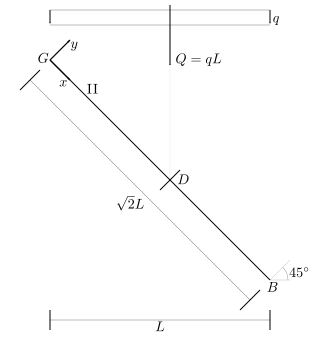
\includegraphics[width=0.45\textwidth]{Immagini/Parte_10/Esercizio10_1_1/Esercizio10_1_5.pdf}
\caption{}
\label{Esercizio10-1-5}
\end{figure}
%--------------------------------------------------------------------------------------------------------------------------------------------------------------
%--------------------------------------------------------------------------------------------------------------------------------------------------------------
\renewcommand{\thefigure}{10.1~-~6}
\begin{figure}[ht]
\centering
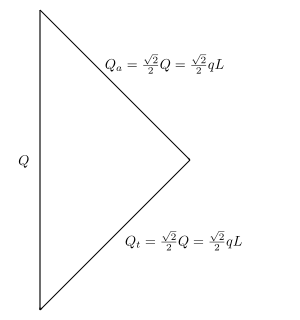
\includegraphics[width=0.5\textwidth]{Immagini/Parte_10/Esercizio10_1_1/Esercizio10_1_6.pdf}
\caption{}
\label{Esercizio10-1-6}
\end{figure}
%--------------------------------------------------------------------------------------------------------------------------------------------------------------
%----------------------------------------------------------------------------------------
La risultante del carico $q$ vale $qL$ ed è verticale. Scomponiamola nelle due direzioni, assiale e trasversale. Questa scomposizione viene riportata esplicitamente nelle figure~\ref{Esercizio10-1-5} e~\ref{Esercizio10-1-6}. Il carico assiale per unità di lunghezza vale dunque: 
%----------------------------------------------------------------------------------------
\begin{equation} \label{equazione10-1-6}
q_{a} = \frac{Q_{a}}{\sqrt{2}L} = \frac{\frac{\sqrt{2}}{2}qL}{\sqrt{2}L} = \frac{q}{2} \tag{10.1.7}
\end{equation}
%----------------------------------------------------------------------------------------
Il carico trasversale vale invece:
%----------------------------------------------------------------------------------------
\begin{equation} \label{equazione10-1-7}
q_{t} = \frac{Q_{t}}{\sqrt{2}L} = \frac{\frac{\sqrt{2}}{2}qL}{\sqrt{2}L} = \frac{q}{2} \tag{10.1.8}
\end{equation}
%----------------------------------------------------------------------------------------
%--------------------------------------------------------------------------------------------------------------------------------------------------------------
\renewcommand{\thefigure}{10.1~-~7}
\begin{figure}[ht]
\centering
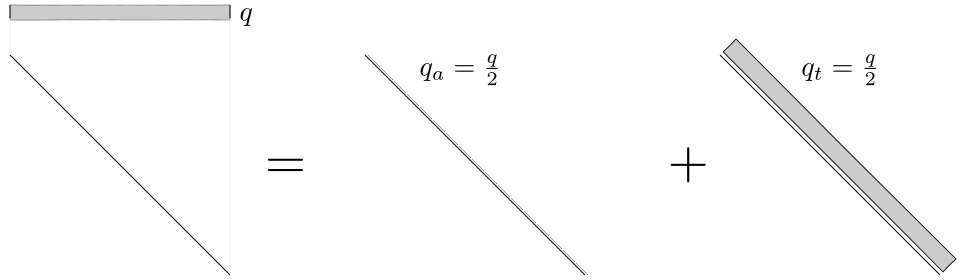
\includegraphics[width=\textwidth]{Immagini/Parte_10/Esercizio10_1_1/Esercizio10_1_7.pdf}
\caption{}
\label{Esercizio10-1-7}
\end{figure}
%--------------------------------------------------------------------------------------------------------------------------------------------------------------
Quindi, abbiamo il quadro rappresentato nella seguente figura~\ref{Esercizio10-1-7}.
%----------------------------------------------------------------------------------------
%----------------------------------------------------------------------------------------
%----------------------------------------------------------------------------------------
%----------------------------------------------------------------------------------------
%----------------------------------------------------------------------------------------
%----------------------------------------------------------------------------------------
%----------------------------------------------------------------------------------------
%----------------------------------------------------------------------------------------
%----------------------------------------------------------------------------------------
%----------------------------------------------------------------------------------------
%----------------------------------------------------------------------------------------